







\section{Comparison with Previous Methods for Guided Sampling}
Below we compare CEP with previous methods for guided sampling.
We show that all previous energy-guided samplers are inexact; and for a special case of the energy function which corresponds to the conditional sampling problem, CEP is a contrastive alternative to classifier guidance.

\begin{figure}[ht]
\vspace{-0.1in}
\centering
\begin{minipage}{0.12\linewidth}
\rotatebox{90}{\scriptsize{Ground Truth}}
\end{minipage}
\begin{minipage}{0.86\linewidth}
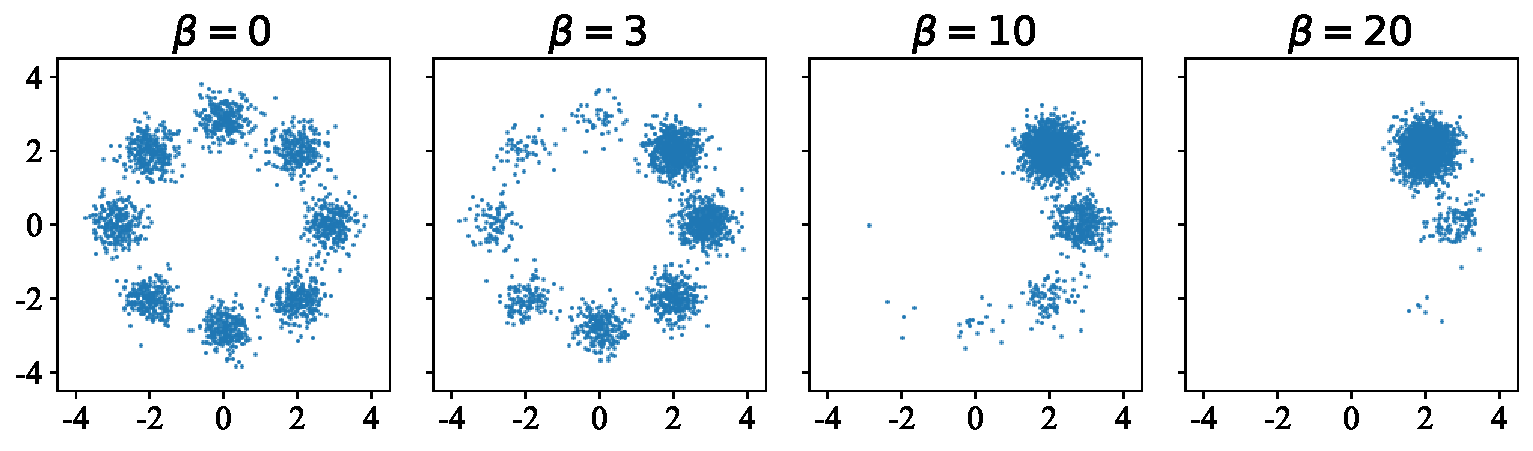
\includegraphics[width=\columnwidth]{pics/toy_scatter/8gaussians_groudtruth_nocolor.pdf}
\end{minipage}

\begin{minipage}{0.06\linewidth}
\rotatebox{90}{\scriptsize{CEP}}
\end{minipage}
\begin{minipage}{0.06\linewidth}
\rotatebox{90}{\scriptsize{(\textbf{ours})}}
\end{minipage}
\begin{minipage}{0.86\linewidth}
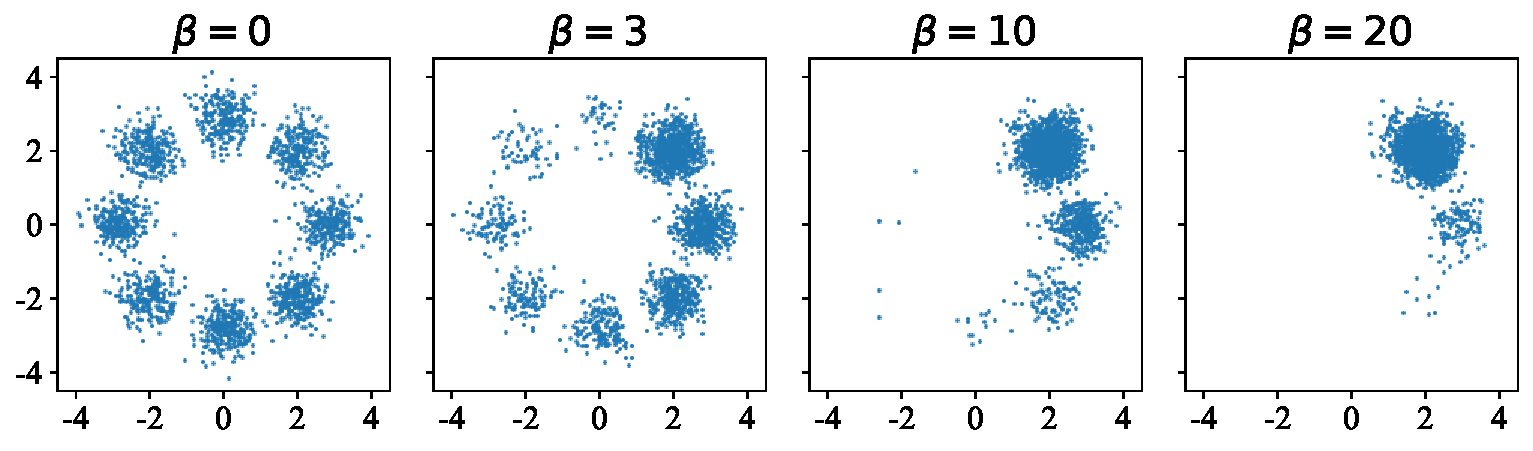
\includegraphics[width=\columnwidth]{pics/toy_scatter/8gaussians_cross_entrophy_nocolor.pdf}
\end{minipage}

\begin{minipage}{0.06\linewidth}
\rotatebox{90}{\scriptsize{MSE}}
\end{minipage}
\begin{minipage}{0.06\linewidth}
\rotatebox{90}{\scriptsize{(\citeauthor{diffuser})}}
\end{minipage}
\begin{minipage}{0.86\linewidth}
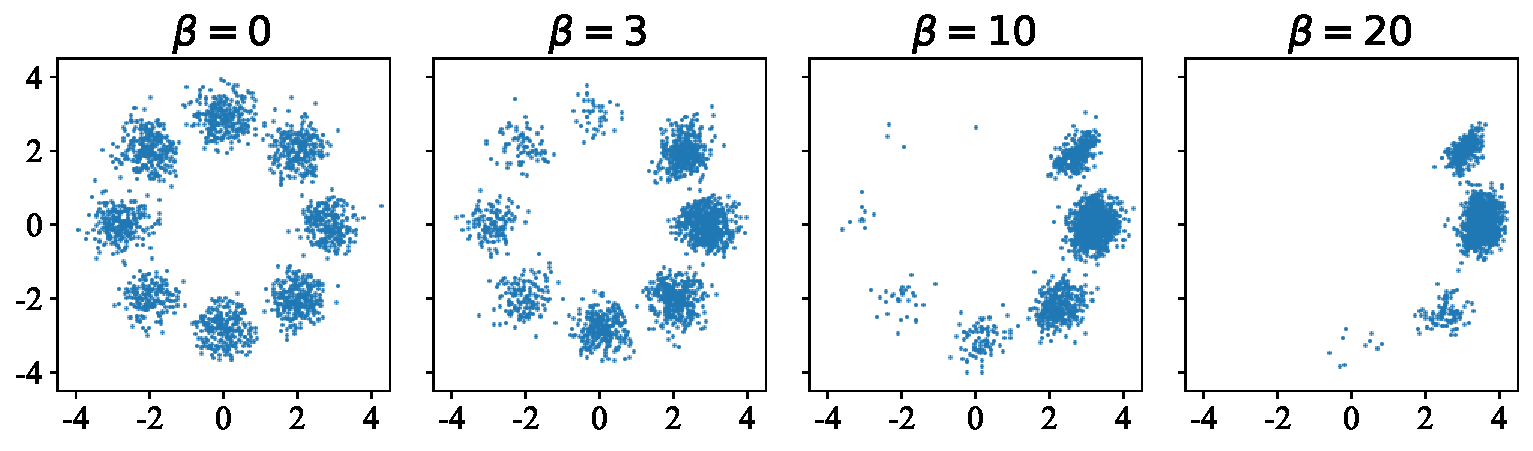
\includegraphics[width=\columnwidth]{pics/toy_scatter/8gaussians_mse_nocolor.pdf}
\end{minipage}

\begin{minipage}{0.06\linewidth}
\rotatebox{90}{\scriptsize{DPS}}
\end{minipage}
\begin{minipage}{0.06\linewidth}
\rotatebox{90}{\scriptsize{(\citeauthor{chung2022diffusion})}}
\end{minipage}
\begin{minipage}{0.86\linewidth}
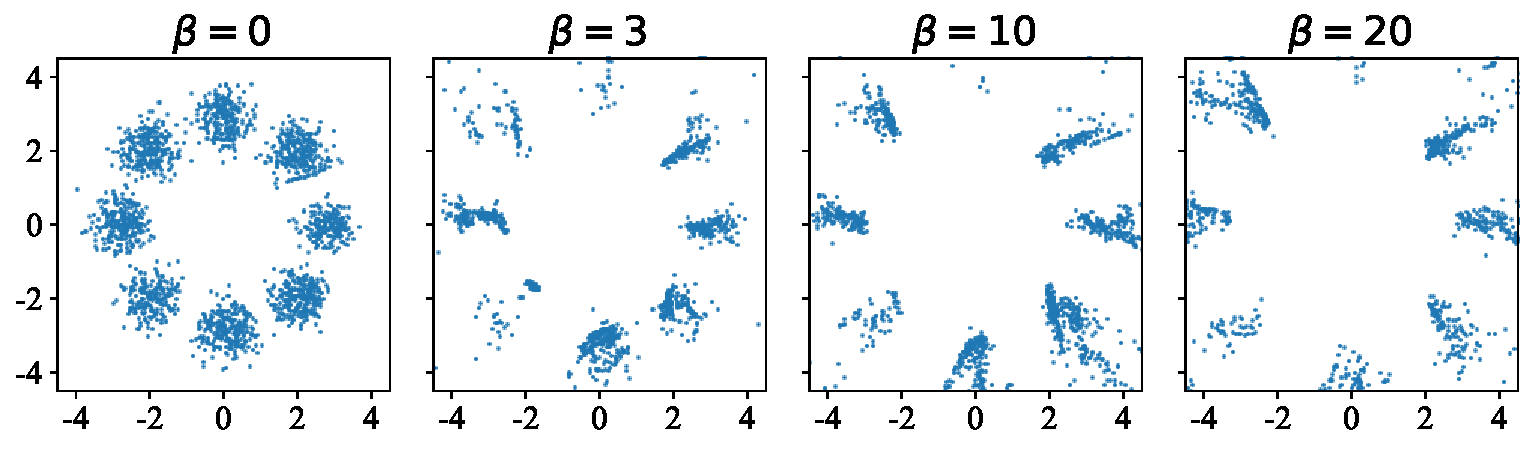
\includegraphics[width=\columnwidth]{pics/toy_scatter/8gaussians_DPS_nocolor.pdf}
\end{minipage}






\caption{
\small{A 2-D example for comparing different energy-guided sampling algorithms, varying different inverse temperature $\beta$.}
}
\label{fig:toy_main}
\end{figure}



\begin{table}[t]
    \vspace{-.1in}
    \centering
    \caption{\small{Comparison between energy-guided sampling algorithms.}}
    \vskip 0.1in
    \begin{small}
    \resizebox{0.48\textwidth}{!}{%
    \begin{tabular}{llc}
    \toprule
    Method & Optimal Solution of Energy &
    Exact Guidance \\
    \midrule
    \vspace{0.03in}
    CEP (ours) & $-\log\E_{q_{0t}(\x_0|\x_t)}\left[e^{-\gE_0(\x_0)}\right]$ & \color{green}{\ding{51}} \\
    \vspace{0.03in}
    MSE & $\E_{q_{0t}(\x_0|\x_t)}[\gE_0(\x_0)]$ & \color{red}{\ding{55}} \\
    DPS & $\gE_0\left(\E_{q_{0t}(\x_0|\x_t)}[\x_0]\right)$ & \color{red}{\ding{55}} \\
    \bottomrule
    \end{tabular}%
    }
    \end{small}
    \label{tab:comparison}
    \vspace{-0.15in}
\end{table}






\subsection{Previous Energy-Guided Samplers are Inexact}
\label{sec:compare_energy}
In this section, we show that previous energy-guided samplers for \eqref{Eq:target_distribution} are all inexact and do not guarantee convergence to $p_0$. 
Without loss of generality, we focus on a fixed time $t\in(0,T]$. 
We summarize the relationship in \cref{tab:comparison}.


\paragraph{MSE for Predicting Energy.}
Many existing energy guidance methods \citep{diffuser,bao2022equivariant} use a mean-square-error (MSE) objective to train an energy model $f_\phi(\x_t, t)$ and use its gradient for energy guidance. The training objective is:
\begin{equation}
\label{Eq:MSE_qt_objective}
    \min_{\phi} \E_{q_{0t}(\x_0, \x_t)} \left[
    \|f_\phi(\x_t, t) - \gE_0(\x_0)\|_2^2
\right]
\end{equation}
Given unlimited model capacity, the optimal $f_\phi$ satisfies:
\begin{equation*}
\begin{split}
    f_\phi^\text{MSE}(\x_t,t) = \E_{q_{0t}(\x_0|\x_t)}\left[
        \gE_0(\x_0)
    \right]
\end{split}
\end{equation*}
However, by \eqref{Eq:intermediate_energy}, the true energy function satisfies
\begin{equation*}
\begin{aligned}
    \gE_t(\x_t) &= -\log \E_{q_{0t}(\x_0|\x_t)}\left[
        e^{-\gE_0(\x_0)} \right] \\
        &\geq \E_{q_{0t}(\x_0|\x_t)}\left[
        \gE_0(\x_0)\right] = f_\phi^\text{MSE}(\x_t,t),
\end{aligned}
\end{equation*}
and the equality only holds when $t=0$. Therefore, the MSE energy function $f_\phi^{\text{MSE}}$ is inexact for all $t>0$. Moreover, we show in Appendix~\ref{appendix:relationship} that the gradient of $f_\phi^{\text{MSE}}$ is also inexact against the true guidance $\nabla_{\x_t}\gE(\x_t)$.

\paragraph{Diffusion Posterior Sampling.}
There also exist some training-free algorithms for energy-guided sampling, such as reconstruction guidance~\citep{ho2022video} and diffusion posterior sampling~\citep{chung2022diffusion}. The basic idea in these methods is to reuse the pretrained diffusion model in the data prediction formulation~\citep{kingma2021variational}:
\begin{equation*}
     \E_{q_{0t}(\x_0|\x_t)}[\x_0] \approx \hat\x_\theta(\x_t,t) \coloneqq \frac{\x_t - \sigma_t\epsilonv_\theta(\x_t,t)}{\alpha_t},
\end{equation*}
and then define the intermediate energy function by:
\begin{equation*}
    f_\theta^{\text{DPS}}(\x_t,t) \coloneqq \gE_0(\hat\x_\theta(\x_t,t)) \approx \gE_0(\E_{q_{0t}(\x_0|\x_t)}[\x_0]).
\end{equation*}
However, we show in Appendix~\ref{appendix:relationship} that $\nabla_{\x_t}f_\theta^{\text{DPS}}\neq \nabla_{\x_t}\gE_t$ and thus it is also inexact.

\paragraph{2-D Example.}
We further compare the different methods for energy-guided sampling on a 2-D example, as shown in Fig.~\ref{fig:toy_main}, and provide more 2-D results in Appendix~\ref{appendix:toy_more}. Experiments show that our method outperforms all referred methods, especially when the inverse temperature $\beta$ is large. 



\subsection{Relationship with Contrastive Learning and Classifier Guidance}
\label{sec:compare_classifier_guidance}
In this section, we consider a special case of our method in which the energy function $\gE_0(\x_0)$ is defined as negative log-likelihood $-\log q_0(c|\x_0)$ for a given conditioning variable $c$ with $\beta=1$. In such case, the desired distribution is:
\begin{equation*}
    p_0(\x_0) \propto q_0(\x_0)q(c|\x_0) \propto q(\x_0|c).
\end{equation*}
Different from the problem we consider in \eqref{Eq:target_distribution} that $p_0(\x_0)$ is hard to draw samples from, here we assume that we can draw samples from $p_0(\x_0)=q_0(\x_0|c)$. Following such an assumption, we prove in Appendix~\ref{appendix:relationship_infonce} that our proposed CEP in \eqref{Eq:infoNCE_energy} is equivalent to
\begin{equation}
\label{Eq:contarstive_condition_loss}
\begin{split}
    \E_{t,\epsilonv^{(1:K)}}\E_{\prod_{i=1}^K q_0(\x_0^{(i)},c^{(i)})}\Bigg[\!\!
    -\sum_{i=1}^K \log \frac{e^{-f_\phi(\x_t^{(i)},c^{(i)},t)}}{\sum_{j=1}^K e^{-f_\phi(\x_t^{(j)},c^{(i)},t)}}
\Bigg],
\end{split}
\end{equation}
where $(\x_0^{(i)}, c^{(i)})$ are $K$ paired data samples from $q_0(\x_0,c)$.
Note that the inner expectation has the same form as the InfoNCE objective~\citep{infoNCE} and is widely used in contrastive learning for multi-modal data, such as CLIP~\citep{radford2021learning} (where $f_\phi$ represents cosine similarity).
Furthermore, \citet{nichol2021glide} uses the above objective and trains a CLIP at each $t$ for text-image pairs and uses its gradient as guidance for text-to-image sampling by diffusion models.
Therefore, such guidance can be considered as a special case of CEP in \eqref{Eq:infoNCE_energy}, under the assumption that we can draw samples from $p_0(\x_0)=q_0(\x_0|c)$.

Moreover, if $c$ is a discrete variable with a total of $M$ possible values (classes). An alternative guided sampling method for sampling from $q_0(\x_0|c)$ is classifier guidance~\citep{diffusion_beat_gan}, which optimize the following objective:
\begin{equation}
\label{Eq:classifier_guidance_loss}
    \E_{t,\epsilonv^{(1:K)}}\E_{\prod_{i=1}^K q_0(\x_0^{(i)},c^{(i)})}\Bigg[\!\!
    -\sum_{i=1}^K \log \frac{e^{-f_\phi(\x_t^{(i)},c^{(i)},t)}}{\sum_{j=1}^M e^{-f_\phi(\x_t^{(i)},c^{(j)},t)}}
\Bigg],
\end{equation}




The most notable difference between \eqref{Eq:contarstive_condition_loss} and \eqref{Eq:classifier_guidance_loss} is the normalizing axes in the training objective's denominator. Classifier guidance aims to \textit{classify conditions} for a given data $\x_t^{(i)}$, so the objective could be understood as a classification loss which is normalized across all $c^{(j)}$. CEP is trying to \textit{compare within data} for a specified condition $c^{(i)}$, so the objective could be understood as a contrastive loss which is normalized across all $\x_t^{(j)}$.

Theoretically, both classifier guidance and CEP could guarantee exact guidance given unlimited data and model capacity. Experimentally, we show in Sec.~\ref{sec:image_exp} that the two methods have quite similar performance.
However, traditional classifier guidance cannot be applied to energy-guided sampling because there does not exist a set of conditions $c$ across which we could normalize, whereas our proposed method can.
We thus conclude that CEP could be considered as a contrastive alternative to classifier guidance for conditional sampling, but is in a more general form that could transfer to the energy-guided sampling problem.


















